\documentclass[12pt, a4paper, twoside]{article}

\usepackage[left = 3cm, top = 3cm, right = 2cm, bottom = 2cm]{geometry}
\usepackage[brazilian]{babel}
\usepackage[utf8]{inputenc}
\usepackage{amsmath, amsfonts, amssymb}
\numberwithin{equation}{subsection}
\usepackage{fancyhdr}
\usepackage{graphicx}
\usepackage{colortbl}
\usepackage{titletoc,titlesec}
\usepackage{setspace}
\usepackage{indentfirst}
\usepackage[colorlinks=true, linkcolor=black, citecolor=black, urlcolor=blue]{hyperref}
\usepackage[alf]{abntex2cite}
\usepackage{multirow}
\usepackage{float}
\usepackage{booktabs}
\usepackage{enumitem}
\usepackage{quoting}
\usepackage{epigraph}
\usepackage{subfigure}
\usepackage{anyfontsize}
\usepackage{caption}
\usepackage{adjustbox}
\usepackage{bm}
\usepackage{siunitx}
\usepackage{listings}
\sisetup{output-decimal-marker = {,}}
\raggedbottom

\newtheorem{teo}{Teorema}[section]
\newtheorem{lema}[teo]{Lema}
\newtheorem{cor}[teo]{Corolário}
\newtheorem{prop}[teo]{Proposição}
\newtheorem{defi}{Definição}
\newtheorem{exem}{Exemplo}

\newcommand{\titulo}{Dinâmica Demográfica no Amapá entre 2000 e 2024: Lexis, Natalidade, Fecundidade e Mortalidade}
\newcommand{\autor}{Felipe Macedo Cordeiro \\ Raphael Borges Leite}
\newcommand{\orientador}{Prof. Dr. Ana Maria Nogales Vasconcelos}

\pagestyle{fancy}
\fancyhf{}
\setlength{\headheight}{16pt}
\fancyhead[RO, LE]{\thepage}
\renewcommand{\sectionmark}[1]{\markboth{#1}{}}

\titlecontents{section}[0cm]{}{\bf\thecontentslabel\ }{}{\titlerule*[.75pc]{.}\contentspage}
\titlecontents{subsection}[0.75cm]{}{\thecontentslabel\ }{}{\titlerule*[.75pc]{.}\contentspage}

\setcounter{secnumdepth}{3}

\DeclareCaptionFormat{myformat}{ \centering \fontsize{10}{12}\selectfont#1#2#3}
\captionsetup{format=myformat}

\begin{document}

\begin{titlepage}
\begin{center}
\begin{figure}[h!]
	\centering
		
\includegraphics[scale = 0.8]{imagens/unb.png}
	\label{fig:unb}
\end{figure}
{\bf Universidade de Brasília \\
\bf Departamento de Estatística}
\vspace{5cm}

\setcounter{page}{0}
\null
\textbf{\titulo}
\vspace{2.5cm}


\vspace{0.2cm}
\textbf{\autor}
\vspace{1.5cm}

\vspace{0.2cm}
\textbf{\orientador}
\end{center}
\vspace{1.5cm}


\begin{flushright}
\begin{minipage}{7.5cm}
\end{minipage}
\end{flushright}

\vspace{5cm}

\begin{center}
{\bf{Brasília} \\ }
\bf{2026}
\end{center}

\end{titlepage}


\pagenumbering{arabic}
\setcounter{page}{2}
\onehalfspacing

\setlength{\parindent}{1.5cm}
\setlength{\parskip}{0.2cm}
\setlength{\intextsep}{0.5cm}

\titlespacing*{\section}{0cm}{0cm}{0.5cm}
\titlespacing*{\subsection}{0cm}{0.5cm}{0.5cm}
\titlespacing*{\subsubsection}{0cm}{0.5cm}{0.5cm}
\titlespacing*{\paragraph}{0cm}{0.5cm}{0.5cm}

\titleformat{\paragraph}{\normalfont\normalsize\bfseries}{\theparagraph}{1em}{}

\pagenumbering{arabic}
\setcounter{page}{3}

\fancyhead[RE, LO]{\nouppercase{\emph\leftmark}}

\tableofcontents
\newpage

\section{Introdução}

Este trabalho tem como objetivo analisar aspectos da dinâmica demográfica do Amapá, considerando o período de 2000 a 2024. O recorte territorial adotado foi a Unidade da Federação Amapá, identificada pelo código 16 do IBGE. A escolha desse recorte permitiu trabalhar, de forma integrada, informações de nascimentos, óbitos, população residente e estrutura por idade e sexo.

Foram utilizados principalmente os dados do SINASC e do SIM, disponibilizados pelo DATASUS, além das projeções populacionais do IBGE -- Revisão 2024 e dos dados do Censo Demográfico de 2022. A partir dessas bases, foram calculados indicadores de sobrevivência na infância, natalidade, fecundidade, reprodução, mortalidade e tábuas de vida.

O trabalho está organizado em três partes principais. A primeira trata do Diagrama de Lexis e da sobrevivência na infância. A segunda analisa os indicadores de natalidade e fecundidade. A terceira apresenta os indicadores de mortalidade, a estrutura de causas de morte e as tábuas de vida. Ao longo das análises, buscou-se manter atenção à qualidade dos dados, aos denominadores utilizados e às limitações dos registros administrativos.

\subsection{Bases de dados utilizadas}

Antes do cálculo dos indicadores, foi definido como recorte territorial o estado do Amapá, código 16 do IBGE. O trabalho utiliza registros de nascidos vivos, óbitos gerais, óbitos fetais e informações populacionais. De forma geral, as bases cobrem o período de 2000 a 2024, embora algumas análises usem recortes menores por causa da janela de observação necessária.

\begin{table}[H]
\centering
\small
\caption{Volumetria geral das bases utilizadas no trabalho.}
\label{tab:volumetria_bases}
\begin{tabular}{p{3.8cm}p{3.5cm}p{5.5cm}}
\toprule
\textbf{Base} & \textbf{Fonte} & \textbf{Dados} \\
\midrule
SINASC & DATASUS/MS & 367.929 nascidos vivos \\
SIM-DO & DATASUS/MS & 68.990 óbitos \\
SIM-DOFET & DATASUS/MS & 4.440 óbitos fetais de residentes no AP \\
Projeções populacionais & IBGE, Revisão 2024 & 19.383 linhas por sexo, idade e ano \\
Censo Demográfico 2022 & IBGE & 1.206 linhas por sexo e idade \\
\bottomrule
\end{tabular}
\end{table}

\begin{table}[H]
\centering
\small
\caption{Principais recortes analíticos utilizados nas questões.}
\label{tab:recortes_analiticos}
\begin{tabular}{p{2cm}p{7.2cm}p{5cm}}
\toprule
\textbf{Questão} & \textbf{Recorte utilizado} & \textbf{Volume analisado} \\
\midrule
Q1 & Coortes de nascidos vivos e óbitos de menores de 5 anos & 299.413 nascidos vivos nas coortes 2000--2019 e 7.044 óbitos de 0 a 4 anos. \\
Q1 & Sobrevivência ao primeiro aniversário & 355.602 nascidos vivos nas coortes 2000--2023 e 7.169 óbitos antes de 1 ano. \\
Q1 & Mortalidade infantil por raça/cor em 2022 e 2023 & 26.563 nascidos vivos e 517 óbitos antes de 1 ano. \\
Q2 & Indicadores de fecundidade em 2010, 2019, 2021, 2022 e 2024 & 71.292 nascidos vivos nos anos selecionados. \\
Q3 & Mortalidade geral em 2010, 2019, 2021, 2022 e 2024 & 17.794 óbitos nos anos selecionados. \\
Q3 & Tábuas de vida para 2010 e 2024 & Taxas específicas de mortalidade por sexo e idade, com tábuas calculadas para homens e mulheres. \\
\bottomrule
\end{tabular}
\end{table}

Essas bases permitem acompanhar três dimensões centrais do trabalho: nascimentos, óbitos e população exposta ao risco. O SINASC fornece os registros de nascidos vivos e as informações maternas e do recém-nascido. O SIM permite observar óbitos por idade, sexo e causa básica. Já os dados do IBGE fornecem os denominadores populacionais necessários para transformar contagens em taxas. Por isso, ao longo do trabalho, os resultados devem ser lidos sempre considerando a qualidade do registro, o recorte territorial e o denominador usado em cada indicador.

\section{Diagrama de Lexis e sobrevivência na infância}

Nesta questão, foram utilizados os nascidos vivos do SINASC e os óbitos do SIM de residentes no Amapá. A análise acompanha coortes de nascimento e óbitos de menores de 5 anos, considerando o pressuposto de população fechada. Isso significa que, para fins de cálculo, não foram consideradas entradas ou saídas por migração. Essa hipótese simplifica a análise, mas deve ser interpretada com cautela, principalmente porque crianças residentes no Amapá podem se deslocar para atendimento em outros estados.

\subsection{Diagrama de Lexis}

O Diagrama de Lexis da Figura \ref{fig:lexis_ap} apresenta os óbitos de menores de 5 anos segundo ano calendário e idade aproximada ao óbito. O eixo horizontal representa o tempo calendário, o eixo vertical representa a idade e as diagonais representam as coortes de nascimento. Assim, cada diagonal acompanha uma geração ao longo do tempo.

\begin{figure}[H]
    \centering
    \caption{Diagrama de Lexis dos óbitos de menores de 5 anos. Amapá, 2000--2024.}
    
\includegraphics[width=0.95\textwidth]{imagens/lexis_ap.png}
    \label{fig:lexis_ap}
\end{figure}

\begin{figure}[H]
    \centering
    \caption{Diagrama de Lexis numérico dos óbitos de menores de 5 anos. Amapá, 2000--2024.}
    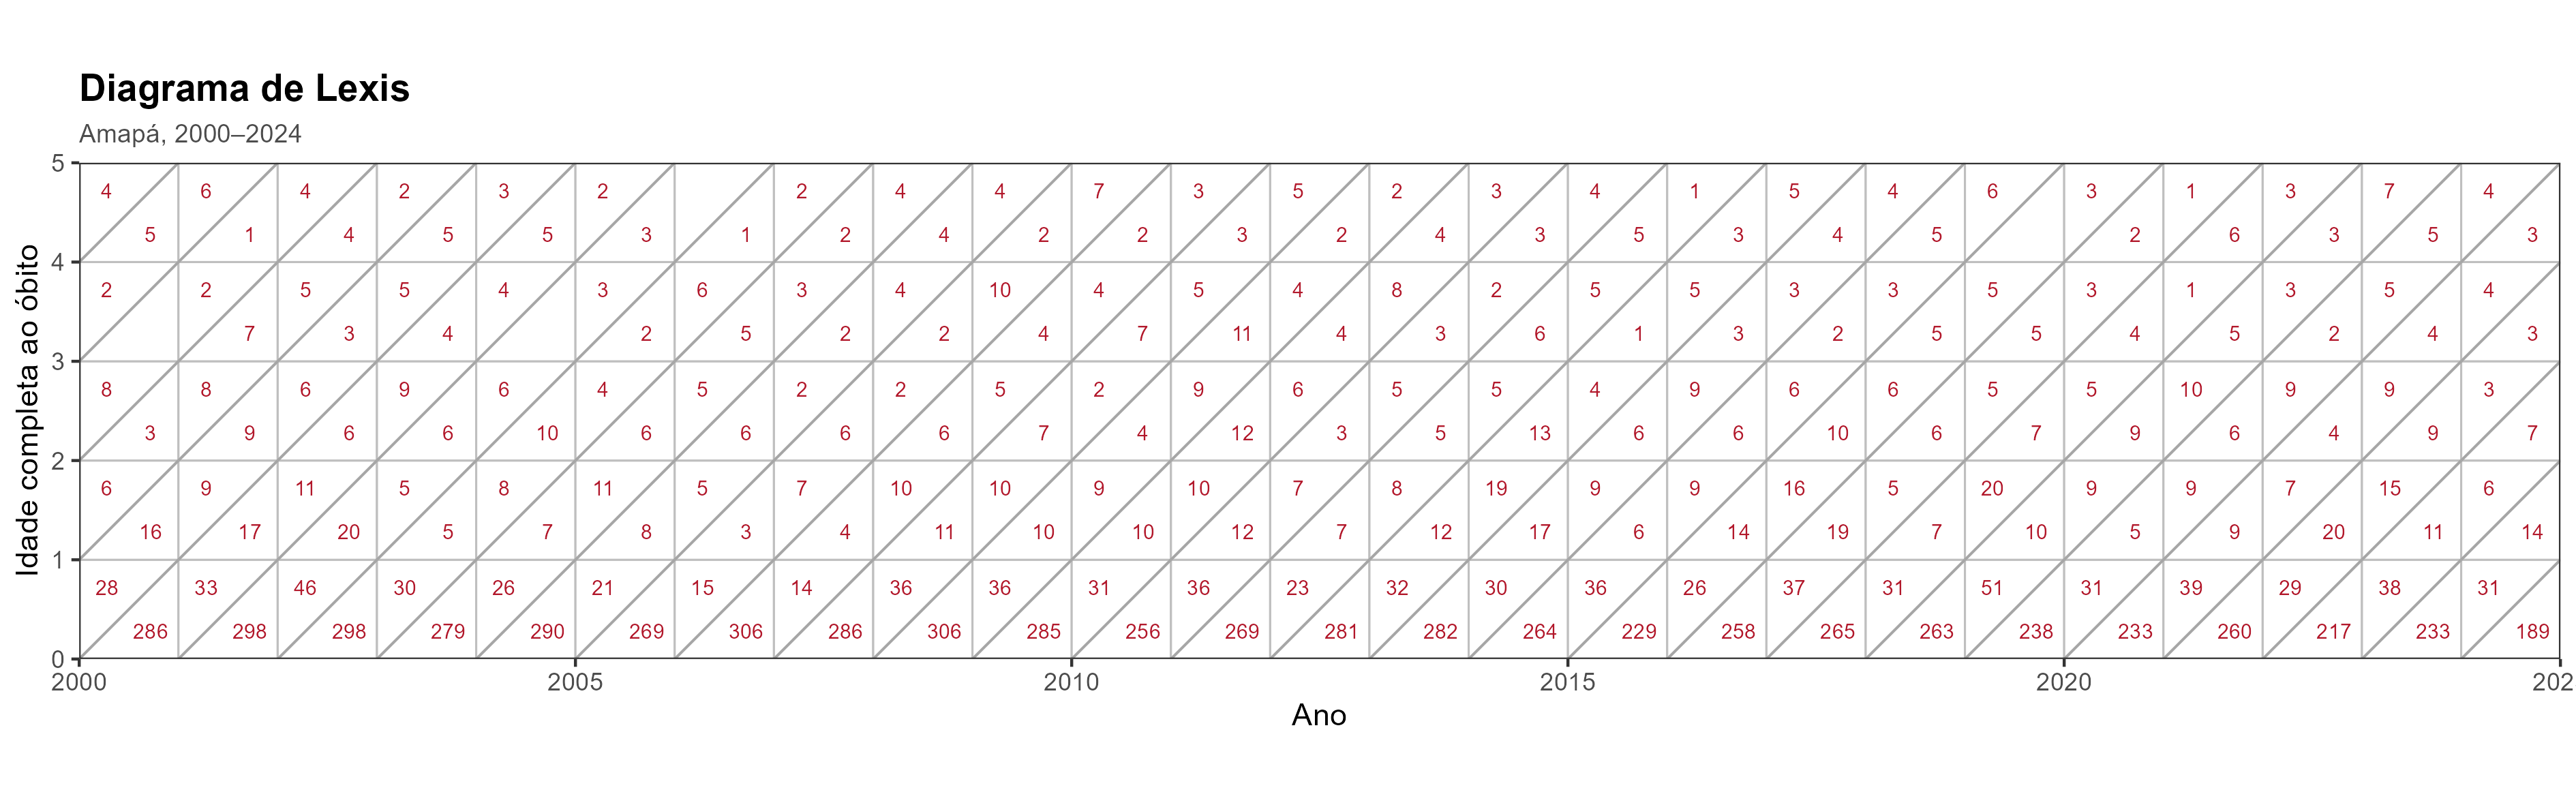
\includegraphics[width=0.95\textwidth]{imagens/lexis_ap_numerico.png}
    \label{fig:lexis_ap_num}
\end{figure}

O gráfico mostra forte concentração de óbitos abaixo de 1 ano de idade, principalmente próximos à idade zero. Esse padrão é esperado, pois o risco de morte é maior no primeiro ano de vida. Entre 1 e 4 anos, os óbitos são menos frequentes e aparecem de forma mais dispersa. A versão numérica do Lexis complementa a leitura visual ao agregar os óbitos nos quadrados idade-ano e separá-los nos triângulos correspondentes às coortes.

\subsection{Sobrevivência até a idade exata de 5 anos}

Para as coortes de nascimento de 2000 a 2019, foi calculada a probabilidade de sobreviver até a idade exata de 5 anos. As coortes posteriores não foram usadas nesse cálculo porque ainda não tinham janela completa de observação até os 5 anos.

\[
{}_{5}q_{0}(Y) = \frac{D_{0-4}(Y)}{B(Y)}
\]

\[
{}_{5}p_{0}(Y) = 1 - {}_{5}q_{0}(Y)
\]

em que $B(Y)$ representa os nascidos vivos da coorte $Y$ e $D_{0-4}(Y)$ representa os óbitos de 0 a 4 anos completos da mesma coorte. Nas tabelas, ${}_{5}q_{0}$ é apresentado por mil nascidos vivos.

\begin{figure}[H]
    \centering
    \caption{Probabilidade de sobreviver até a idade exata de 5 anos. Amapá, coortes 2000--2019.}
    
\includegraphics[width=0.85\textwidth]{imagens/grafico_5p0_ap.png}
    \label{fig:5p0_ap}
\end{figure}

\begin{table}[H]
\centering
\scriptsize
\caption{Probabilidade de sobreviver até a idade exata de 5 anos. Amapá, coortes 2000--2019.}
\label{tab:5p0_ap}
\resizebox{\textwidth}{!}{%
\begin{tabular}{rrrrr}
\toprule
\textbf{Coorte} & \textbf{Nascidos vivos} & \textbf{Óbitos 0--4} & \textbf{${}_{5}q_{0}$ por mil} & \textbf{${}_{5}p_{0}$} \\
\midrule
2000 & 14.238 & 375 & 26,3 & 0,974 \\
2001 & 14.609 & 385 & 26,4 & 0,974 \\
2002 & 14.196 & 366 & 25,8 & 0,974 \\
2003 & 14.764 & 346 & 23,4 & 0,977 \\
2004 & 13.971 & 345 & 24,7 & 0,975 \\
2005 & 14.205 & 322 & 22,7 & 0,977 \\
2006 & 14.714 & 357 & 24,3 & 0,976 \\
2007 & 14.425 & 372 & 25,8 & 0,974 \\
2008 & 15.105 & 390 & 25,8 & 0,974 \\
2009 & 14.298 & 369 & 25,8 & 0,974 \\
2010 & 15.008 & 328 & 21,9 & 0,978 \\
2011 & 15.114 & 329 & 21,8 & 0,978 \\
2012 & 14.895 & 373 & 25,0 & 0,975 \\
2013 & 15.710 & 362 & 23,0 & 0,977 \\
2014 & 16.271 & 339 & 20,8 & 0,979 \\
2015 & 15.750 & 314 & 19,9 & 0,980 \\
2016 & 15.521 & 341 & 22,0 & 0,978 \\
2017 & 15.399 & 347 & 22,5 & 0,977 \\
2018 & 15.864 & 370 & 23,3 & 0,977 \\
2019 & 15.356 & 314 & 20,4 & 0,980 \\
\bottomrule
\end{tabular}
}
\end{table}

A sobrevivência até os 5 anos permaneceu elevada em todas as coortes, variando aproximadamente entre 97,4\% e 98,0\%. Em termos complementares, a mortalidade antes dos 5 anos variou entre cerca de 19,9 e 26,4 óbitos por mil nascidos vivos. Apesar de algumas oscilações, há melhora em relação às primeiras coortes dos anos 2000.

\subsection{Sobrevivência ao primeiro aniversário}

Também foi calculada a probabilidade de sobreviver ao primeiro aniversário para as coortes de 2000 a 2023. Neste caso, foram considerados os óbitos ocorridos antes de completar 1 ano de idade.

\[
{}_{1}q_{0}(Y) = \frac{D_{<1}(Y)}{B(Y)}
\]

\[
{}_{1}p_{0}(Y) = 1 - {}_{1}q_{0}(Y)
\]

Nas tabelas, ${}_{1}q_{0}$ é apresentado por mil nascidos vivos, enquanto ${}_{1}p_{0}$ é apresentado como probabilidade.

\begin{figure}[H]
    \centering
    \caption{Probabilidade de sobreviver ao primeiro aniversário. Amapá, coortes 2000--2023.}
    
\includegraphics[width=0.85\textwidth]{imagens/grafico_1p0_ap.png}
    \label{fig:1p0_ap}
\end{figure}

\begin{table}[H]
\centering
\scriptsize
\caption{Probabilidade de sobreviver ao primeiro aniversário. Amapá, coortes 2000--2023.}
\label{tab:1p0_ap}
\resizebox{\textwidth}{!}{%
\begin{tabular}{rrrrr}
\toprule
\textbf{Coorte} & \textbf{Nascidos vivos} & \textbf{Óbitos $<1$ ano} & \textbf{${}_{1}q_{0}$ por mil} & \textbf{${}_{1}p_{0}$} \\
\midrule
2000 & 14.238 & 318 & 22,3 & 0,978 \\
2001 & 14.609 & 343 & 23,5 & 0,977 \\
2002 & 14.196 & 327 & 23,0 & 0,977 \\
2003 & 14.764 & 302 & 20,5 & 0,980 \\
2004 & 13.971 & 310 & 22,2 & 0,978 \\
2005 & 14.205 & 283 & 19,9 & 0,980 \\
2006 & 14.714 & 319 & 21,7 & 0,978 \\
2007 & 14.425 & 322 & 22,3 & 0,978 \\
2008 & 15.105 & 339 & 22,4 & 0,978 \\
2009 & 14.298 & 312 & 21,8 & 0,978 \\
2010 & 15.008 & 289 & 19,3 & 0,981 \\
2011 & 15.114 & 287 & 19,0 & 0,981 \\
2012 & 14.895 & 310 & 20,8 & 0,979 \\
2013 & 15.710 & 308 & 19,6 & 0,980 \\
2014 & 16.271 & 295 & 18,1 & 0,982 \\
2015 & 15.750 & 255 & 16,2 & 0,984 \\
2016 & 15.521 & 295 & 19,0 & 0,981 \\
2017 & 15.399 & 294 & 19,1 & 0,981 \\
2018 & 15.864 & 314 & 19,8 & 0,980 \\
2019 & 15.356 & 269 & 17,5 & 0,982 \\
2020 & 14.633 & 272 & 18,6 & 0,981 \\
2021 & 14.993 & 289 & 19,3 & 0,981 \\
2022 & 13.615 & 255 & 18,7 & 0,981 \\
2023 & 12.948 & 262 & 20,2 & 0,980 \\
\bottomrule
\end{tabular}
}
\end{table}

A comparação entre ${}_{1}q_{0}$ e ${}_{5}q_{0}$ mostra que a maior parte dos óbitos antes dos 5 anos ocorre no primeiro ano de vida. Esse resultado também aparece no Diagrama de Lexis, pela concentração de pontos na parte inferior do gráfico. A coorte de 2023 deve ser lida com atenção, pois parte dos seus óbitos antes do primeiro aniversário ocorre em 2024, ano ainda sujeito a atualização nas bases do DATASUS.

\subsection{Mortalidade antes do primeiro aniversário por raça/cor}

Para 2022 e 2023, foi calculada a probabilidade de morrer antes do primeiro aniversário segundo raça/cor. O cálculo seguiu a mesma lógica da mortalidade infantil, separando nascimentos e óbitos por categoria de raça/cor.

\[
{}_{1}q_{0,r}(Y) = \frac{D_{<1,r}(Y)}{B_{r}(Y)}
\]

em que $r$ representa a categoria de raça/cor.

\begin{figure}[H]
    \centering
    \caption{Probabilidade de morrer antes do primeiro aniversário segundo raça/cor. Amapá, coortes 2022 e 2023.}
    
\includegraphics[width=0.85\textwidth]{imagens/grafico_q0_raca_ap.png}
    \label{fig:q0_raca_ap}
\end{figure}

\begin{table}[H]
\centering
\scriptsize
\caption{Probabilidade de morrer antes do primeiro aniversário segundo raça/cor. Amapá, 2022 e 2023.}
\label{tab:q0_raca_ap}
\resizebox{\textwidth}{!}{%
\begin{tabular}{llrrrl}
\toprule
\textbf{Coorte} & \textbf{Raça/cor} & \textbf{Nascidos vivos} & \textbf{Óbitos $<1$ ano} & \textbf{${}_{1}q_{0}$ por mil} & \textbf{Observação} \\
\midrule
2022 & Branca   & 1.609  & 35  & 21,8  &  \\
2022 & Preta    & 886    & 2   & 2,3   & $n < 10$ \\
2022 & Amarela  & 22     & 2   & 90,9  & $n < 10$ \\
2022 & Parda    & 10.720 & 163 & 15,2  &  \\
2022 & Indígena & 293    & 10  & 34,1  &  \\
2022 & Ignorada & 85     & 43  & 505,9 & raça/cor ignorada \\
2023 & Branca   & 1.589  & 50  & 31,5  &  \\
2023 & Preta    & 999    & 4   & 4,0   & $n < 10$ \\
2023 & Amarela  & 35     & 0   & 0,0   & $n < 10$ \\
2023 & Parda    & 9.979  & 178 & 17,8  &  \\
2023 & Indígena & 295    & 9   & 30,5  & $n < 10$ \\
2023 & Ignorada & 51     & 21  & 411,8 & raça/cor ignorada \\
\bottomrule
\end{tabular}
}
\end{table}

Algumas categorias têm menos de 10 óbitos, o que torna as estimativas instáveis. Além disso, a categoria ignorada apresentou valores elevados, indicando problema de preenchimento e de comparabilidade entre SIM e SINASC. No período analisado, a raça/cor ignorada representou 12,4\% dos óbitos infantis no SIM e apenas 0,5\% dos nascimentos no SINASC.

Entre as categorias com maior volume de eventos, pardos apresentaram valores menores que brancos e indígenas nos dois anos analisados. Ainda assim, esses resultados devem ser lidos como uma análise exploratória, porque dependem da qualidade da informação de raça/cor e de números pequenos em algumas categorias.

\subsection{Comentários}

Os resultados da Questão 1 são coerentes entre si. O Diagrama de Lexis mostra concentração dos óbitos nos primeiros meses de vida, e as probabilidades calculadas confirmam que a maior parte da mortalidade antes dos 5 anos ocorre antes do primeiro aniversário.

A sobrevivência até 1 ano e até 5 anos é elevada nas coortes analisadas, com melhora geral em relação ao início dos anos 2000. A análise por raça/cor acrescenta uma dimensão importante, mas depende fortemente da qualidade do preenchimento das bases.

As principais limitações são o uso do pressuposto de população fechada, a possibilidade de sub-registro de óbitos e a diferença de preenchimento da raça/cor entre SINASC e SIM.

\section{Fecundidade e Natalidade}

\subsection{Indicadores de fecundidade}

Nesta questão foram calculados indicadores de fecundidade para o Amapá nos anos de 2010, 2019, 2021, 2022 e 2024. Os nascidos vivos foram obtidos no SINASC/DATASUS \cite{datasus2026} e os denominadores populacionais vieram das projeções populacionais do IBGE -- Revisão 2024 \cite{ibge2024}. Foram consideradas mulheres em idade reprodutiva, de 15 a 49 anos.

As principais medidas utilizadas foram a Taxa Bruta de Natalidade (TBN), a Taxa de Fecundidade Geral (TFG), as Taxas Específicas de Fecundidade por idade (${}_nf_x$), as taxas específicas considerando apenas nascidos vivos do sexo feminino, a Taxa de Fecundidade Total (TFT), a Taxa Bruta de Reprodução (TBR) e a Taxa Líquida de Reprodução (TLR).

A Taxa Bruta de Natalidade relaciona o total de nascidos vivos com a população média ou população de referência do ano:

\begin{equation}
\label{eq:tbn}
TBN = \frac{\mathrm{NV}}{\bar{P}} \times 1000
\end{equation}

A Taxa de Fecundidade Geral considera apenas a população feminina em idade reprodutiva:

\begin{equation}
\label{eq:tfg}
TFG = \frac{\mathrm{NV}}{\bar{P}_{f,15-49}} \times 1000
\end{equation}

As Taxas Específicas de Fecundidade por idade foram calculadas para cada grupo etário da mãe:

\begin{equation}
\label{eq:nfx}
{}_nf_x = \frac{{}_n\mathrm{NV}_x}{{}_n\bar{P}_{f,x}} \times 1000
\end{equation}

Também foram calculadas as taxas específicas considerando apenas os nascidos vivos do sexo feminino:

\begin{equation}
\label{eq:nfx_fem}
{}_nf_x^{fem} = \frac{{}_n\mathrm{NV}_x^{fem}}{{}_n\bar{P}_{f,x}} \times 1000
\end{equation}

A Taxa de Fecundidade Total foi obtida a partir da soma das taxas específicas de fecundidade. Como os grupos etários são quinquenais, foi utilizado $n=5$:

\begin{equation}
\label{eq:tft}
TFT = 5 \times \sum_x \frac{{}_nf_x}{1000}
\end{equation}

A Taxa Bruta de Reprodução considera apenas os nascidos vivos do sexo feminino:

\begin{equation}
\label{eq:tbr}
TBR = 5 \times \sum_x \frac{{}_nf_x^{fem}}{1000}
\end{equation}

Por fim, a Taxa Líquida de Reprodução incorpora a sobrevivência feminina nas idades reprodutivas, por meio da função ${}_nL_x$ da tábua de vida:

\begin{equation}
\label{eq:tlr}
TLR = 5 \times \sum_x \left(\frac{{}_nf_x^{fem}}{1000}\right) \times \frac{{}_nL_x}{5l_0}
\end{equation}

em que $\mathrm{NV}$ representa o total de nascidos vivos, $\bar{P}$ a população média ou população de referência do ano, $\bar{P}_{f,15-49}$ a população feminina de 15 a 49 anos, ${}_n\mathrm{NV}_x$ os nascidos vivos de mães no grupo etário $x$ a $x+n$, ${}_n\mathrm{NV}_x^{fem}$ os nascidos vivos do sexo feminino nesse mesmo grupo etário, ${}_n\bar{P}_{f,x}$ a população feminina do grupo etário e ${}_nL_x/(5l_0)$ o fator médio de sobrevivência feminina no intervalo etário.

\begin{table}[H]
\centering
\small
\caption{Indicadores de fecundidade e reprodução. Amapá, anos selecionados.}
\label{tab:q2_indicadores}
\resizebox{\textwidth}{!}{%
\begin{tabular}{rrrrrrrr}
\toprule
\textbf{Ano} & \textbf{TBN} & \textbf{TFG} & \textbf{TFT} & \textbf{TBR} & \textbf{TLR} & \textbf{Nascidos vivos} & \textbf{Mulheres 15--49} \\
\midrule
2010 & 21,85 & 79,94 & 2,308 & 1,139 & 1,097 & 15.008 & 187.750 \\
2019 & 19,70 & 69,70 & 2,174 & 1,053 & 1,019 & 15.355 & 220.313 \\
2021 & 18,95 & 67,24 & 2,129 & 1,036 & 1,000 & 14.988 & 222.908 \\
2022 & 17,11 & 60,92 & 1,944 & 0,942 & 0,910 & 13.614 & 223.468 \\
2024 & 15,35 & 54,91 & 1,779 & 0,874 & 0,847 & 12.327 & 224.481 \\
\bottomrule
\end{tabular}
}
\end{table}

A TBN, a TFG e as taxas específicas são expressas por mil. Já a TFT, a TBR e a TLR são interpretadas como número médio de filhos ou filhas por mulher. Os resultados indicam queda da fecundidade no período analisado. A TFT, calculada pela Equação~\eqref{eq:tft}, passou de 2,308 filhos por mulher em 2010 para 1,779 em 2024, ficando abaixo do nível de reposição populacional. A TLR, definida na Equação~\eqref{eq:tlr}, também ficou abaixo de 1 a partir de 2022, indicando que, mantidas as condições de fecundidade e mortalidade observadas, a geração de mulheres não seria integralmente reposta por filhas.

\begin{figure}[H]
    \centering
    \caption{Taxas específicas de fecundidade por grupo etário. Amapá, anos selecionados.}
    
\includegraphics[width=0.85\textwidth]{imagens/tef_ap.png}
    \label{fig:q2_tef}
\end{figure}

As curvas de ${}_nf_x$, calculadas conforme a Equação~\eqref{eq:nfx}, mostram concentração da fecundidade nas idades de 20 a 29 anos. Também se observa queda em praticamente todos os grupos etários, especialmente entre mulheres mais jovens. Esse comportamento é compatível com a tendência de redução da fecundidade brasileira discutida por \citeonline{mirandaribeiro2019}, associada a mudanças no padrão reprodutivo, maior escolarização e adiamento da maternidade.

\subsection{Comparação com o Censo 2022}

Para 2022, os indicadores também foram recalculados utilizando a população recenseada no Censo Demográfico de 2022. Como o Censo apresentou população menor que a projeção usada como denominador, as taxas calculadas com o Censo ficaram mais elevadas.

\begin{table}[H]
\centering
\small
\caption{Indicadores de fecundidade em 2022 segundo o denominador populacional.}
\label{tab:q2_censo_proj}
\resizebox{\textwidth}{!}{%
\begin{tabular}{lrrrrrrr}
\toprule
\textbf{Denominador} & \textbf{TBN} & \textbf{TFG} & \textbf{TFT} & \textbf{TBR} & \textbf{TLR} & \textbf{Pop. total} & \textbf{Mulheres 15--49} \\
\midrule
Projeção IBGE Rev. 2024 & 17,11 & 60,92 & 1,944 & 0,942 & 0,910 & 795.457 & 223.468 \\
Censo 2022 & 18,55 & 65,41 & 2,100 & 1,017 & 0,983 & 733.759 & 208.149 \\
\bottomrule
\end{tabular}
}
\end{table}

A comparação mostra a importância do denominador utilizado. Com a população do Censo, a TFT de 2022 fica próxima de 2,1 filhos por mulher, enquanto com a projeção fica em 1,944. Portanto, a diferença não está nos nascidos vivos, que são os mesmos, mas no tamanho da população feminina usada como base de cálculo.

\begin{figure}[H]
    \centering
    \caption{Taxas específicas de fecundidade em 2022 segundo o denominador utilizado.}
    
\includegraphics[width=0.78\textwidth]{imagens/tef_comp_2022_ap.png}
    \label{fig:q2_tef_2022}
\end{figure}

\subsection{Reprodução}

A Taxa Bruta de Reprodução (TBR), definida na Equação~\eqref{eq:tbr}, considera apenas os nascidos vivos do sexo feminino por idade da mãe. Já a Taxa Líquida de Reprodução (TLR), definida na Equação~\eqref{eq:tlr}, ajusta esse resultado pela sobrevivência feminina até as idades reprodutivas, utilizando a função ${}_nL_x$ da tábua de vida.

Enquanto a TBR indica o número médio de filhas que uma mulher teria ao longo do período reprodutivo, mantidas as taxas de fecundidade observadas, a TLR incorpora também o efeito da mortalidade feminina antes e durante as idades reprodutivas.

\begin{figure}[H]
    \centering
    \caption{Taxa Bruta e Taxa Líquida de Reprodução. Amapá, anos selecionados.}
    
\includegraphics[width=0.78\textwidth]{imagens/tbr_tlr_ap.png}
    \label{fig:q2_tbr_tlr}
\end{figure}

A diferença entre TBR e TLR foi pequena, o que indica que a mortalidade feminina antes ou durante as idades reprodutivas não altera fortemente o resultado. O principal fator para a queda da TLR é, portanto, a própria redução da fecundidade.

\subsection{Associação entre idade e escolaridade da mãe}

Para 2024, foi analisada a relação entre grupo de idade da mãe e escolaridade por meio de uma tabela de contingência. Foram apresentadas as frequências absolutas e os percentuais por linha, isto é, a distribuição da escolaridade dentro de cada grupo etário.

\begin{table}[H]
\centering
\scriptsize
\caption{Idade da mãe e escolaridade. SINASC 2024, Amapá.}
\label{tab:q2_idade_esc}
\resizebox{\textwidth}{!}{%
\begin{tabular}{lrrrr}
\toprule
\textbf{Grupo de idade} & \textbf{Nenhuma} & \textbf{Fund. incompleto} & \textbf{Médio/Fund. completo} & \textbf{Superior} \\
\midrule
$<20$ & 2 (0,1\%) & 560 (25,9\%) & 1.567 (72,5\%) & 30 (1,4\%) \\
20--24 & 6 (0,2\%) & 571 (17,7\%) & 2.275 (70,4\%) & 378 (11,7\%) \\
25--29 & 4 (0,1\%) & 463 (16,0\%) & 1.713 (59,2\%) & 711 (24,6\%) \\
30--34 & 7 (0,3\%) & 312 (14,6\%) & 1.146 (53,7\%) & 669 (31,3\%) \\
35+ & 27 (1,4\%) & 369 (19,3\%) & 892 (46,7\%) & 620 (32,5\%) \\
\bottomrule
\end{tabular}
}
\end{table}

Como medida descritiva, foi utilizada a diferença entre proporções em pontos percentuais. Essa escolha é adequada porque o objetivo aqui é comparar a distribuição observada entre os grupos, sem transformar a análise em um teste de hipótese.

\[
\Delta p = p_1 - p_0
\]

No caso da escolaridade superior, a proporção foi de 1,4\% entre mães com menos de 20 anos e de 32,5\% entre mães de 35 anos ou mais. A diferença foi, portanto, de 31,1 pontos percentuais. Esse resultado indica associação descritiva entre idade e escolaridade: mães em idades mais elevadas apresentam maior participação relativa no ensino superior.

\begin{figure}[H]
    \centering
    \caption{Distribuição percentual da escolaridade segundo grupo de idade da mãe. SINASC 2024, Amapá.}
    
\includegraphics[width=0.78\textwidth]{imagens/heat_idade_esc_2024.png}
    \label{fig:q2_idade_esc}
\end{figure}

\subsection{Associação entre tipo de parto e escolaridade da mãe}

Também foi analisada a relação entre tipo de parto e escolaridade da mãe. A Tabela \ref{tab:q2_parto_esc} apresenta a tabela de contingência com frequências absolutas e percentuais por linha.

\begin{table}[H]
\centering
\scriptsize
\caption{Tipo de parto e escolaridade da mãe. SINASC 2024, Amapá.}
\label{tab:q2_parto_esc}
\resizebox{\textwidth}{!}{%
\begin{tabular}{lrrrr}
\toprule
\textbf{Tipo de parto} & \textbf{Nenhuma} & \textbf{Fund. incompleto} & \textbf{Médio/Fund. completo} & \textbf{Superior} \\
\midrule
Cesárea & 15 (0,3\%) & 684 (12,6\%) & 3.131 (57,8\%) & 1.584 (29,3\%) \\
Vaginal & 31 (0,4\%) & 1.591 (23,0\%) & 4.461 (64,6\%) & 827 (12,0\%) \\
\bottomrule
\end{tabular}
}
\end{table}

A partir da mesma tabela de contingência, também foi calculada a proporção de cesáreas dentro de cada grupo de escolaridade. Entre mães com ensino fundamental incompleto, 30,1\% dos partos foram cesáreos. Entre mães com ensino superior, essa proporção foi de 65,7\%. A diferença foi de 35,6 pontos percentuais.

Esse resultado mostra uma associação descritiva importante entre escolaridade e tipo de parto: quanto maior a escolaridade, maior a participação relativa dos partos cesáreos. Como se trata de uma análise descritiva com dados populacionais do SINASC, a interpretação foi baseada nas proporções observadas e nas diferenças em pontos percentuais.

\begin{figure}[H]
    \centering
    \caption{Distribuição da escolaridade segundo tipo de parto. SINASC 2024, Amapá.}
    
\includegraphics[width=0.72\textwidth]{imagens/parto_esc_2024.png}
    \label{fig:q2_parto_esc}
\end{figure}

\subsection{Comentários}

A Questão 2 mostra queda consistente da fecundidade no Amapá entre 2010 e 2024. A redução aparece tanto nas taxas específicas por idade quanto na TFT, na TBR e na TLR. Em 2022, a escolha do denominador populacional altera os resultados, especialmente a TFT, mostrando a importância de explicitar se foram usadas projeções ou população recenseada.

Para 2024, a análise das tabelas de contingência indica associação descritiva entre idade, escolaridade da mãe e tipo de parto. Mães mais velhas apresentaram maior proporção de ensino superior, e mães com ensino superior apresentaram maior proporção de partos cesáreos. Esses resultados foram interpretados por meio de frequências relativas e diferenças em pontos percentuais.

\section{Mortalidade}

\subsection{Procedimentos}

Nesta questão foram utilizados os microdados do SIM/DATASUS para óbitos de residentes no Amapá \cite{datasus2026} e as populações projetadas pelo IBGE -- Revisão 2024 \cite{ibge2024}. Os anos analisados foram 2010, 2019, 2021, 2022 e 2024.

Foram calculadas a Taxa Bruta de Mortalidade (TBM), as taxas específicas de mortalidade por sexo e idade (${}_nM_x$), indicadores de mortalidade infantil e perinatal, a estrutura de causas de morte e tábuas de vida abreviadas para 2010 e 2024.

A Taxa Bruta de Mortalidade foi calculada por:

\[
TBM = \frac{D}{P} \times 1000
\]

em que $D$ é o total de óbitos no ano e $P$ é a população projetada no mesmo ano.

As taxas específicas de mortalidade foram calculadas por:

\[
{}_nM_x = \frac{{}_nD_x}{{}_nP_x} \times 1000
\]

em que ${}_nD_x$ representa os óbitos no grupo etário e ${}_nP_x$ representa a população do mesmo grupo. Neste caso, ${}_nM_x$ é apresentado por mil habitantes.

\subsection{Taxa Bruta e Taxas Específicas de Mortalidade}

A Tabela \ref{tab:tbm_q3} apresenta a Taxa Bruta de Mortalidade para os anos selecionados. A TBM aumenta entre 2010 e 2021, com pico em 2021, ano marcado pela pandemia de COVID-19. Em 2022 e 2024, a taxa diminui em relação a 2021, mas permanece acima do valor observado em 2010.

\begin{table}[H]
\centering
\small
\caption{Taxa Bruta de Mortalidade. Amapá, anos selecionados.}
\label{tab:tbm_q3}
\begin{tabular}{rrrr}
\toprule
\textbf{Ano} & \textbf{Óbitos} & \textbf{População projetada} & \textbf{TBM por mil} \\
\midrule
2010 & 2.276 & 686.987 & 3,31 \\
2019 & 3.407 & 779.468 & 4,37 \\
2021 & 4.578 & 790.871 & 5,79 \\
2022 & 3.735 & 795.457 & 4,70 \\
2024 & 3.798 & 802.837 & 4,73 \\
\bottomrule
\end{tabular}
\end{table}

As taxas específicas por sexo e idade mostram o padrão esperado: mortalidade mais elevada no primeiro ano de vida, queda nas idades infantis e aumento progressivo nas idades adultas e idosas. Também se observa maior mortalidade masculina em quase todos os grupos etários, principalmente nas idades jovens e adultas.

\begin{figure}[H]
    \centering
    \caption{Taxas específicas de mortalidade por sexo e grupo etário. Amapá, anos selecionados.}
    
\includegraphics[width=0.95\textwidth]{imagens/nmx_painel_ap.png}
    \label{fig:nmx_painel_q3}
\end{figure}

\subsection{Mortalidade Infantil e Perinatal}

A Taxa de Mortalidade Infantil (TMI) foi calculada conforme solicitado no enunciado: média dos óbitos infantis de 2022 a 2024 no numerador e nascidos vivos de 2023 no denominador.

\[
TMI = \frac{\overline{D}_{<1,\,2022-2024}}{NV_{2023}} \times 1000
\]

\begin{table}[H]
\centering
\small
\caption{Taxa de Mortalidade Infantil, total e por sexo. Amapá.}
\label{tab:tmi_q3}
\begin{tabular}{lrrr}
\toprule
\textbf{Sexo} & \textbf{Média de óbitos infantis} & \textbf{NV 2023} & \textbf{TMI por mil} \\
\midrule
Total & 238,3 & 12.948 & 18,41 \\
Masculino & 128,7 & 6.637 & 19,39 \\
Feminino & 107,7 & 6.310 & 17,06 \\
\bottomrule
\end{tabular}
\end{table}

A TMI masculina foi maior que a feminina, padrão comum em estudos de mortalidade infantil. A decomposição mostra maior peso dos óbitos neonatais precoces, isto é, ocorridos de 0 a 6 dias de vida.

\begin{table}[H]
\centering
\small
\caption{Componentes da mortalidade infantil. Amapá.}
\label{tab:componentes_tmi_q3}
\resizebox{\textwidth}{!}{%
\begin{tabular}{lrr}
\toprule
\textbf{Componente} & \textbf{Média de óbitos 2022--2024} & \textbf{Taxa por mil} \\
\midrule
Neonatal precoce (0--6 dias) & 112,3 & 8,68 \\
Neonatal tardio (7--27 dias) & 32,0 & 2,47 \\
Neonatal total (0--27 dias) & 144,3 & 11,15 \\
Pós-neonatal (28 dias--menos de 1 ano) & 94,0 & 7,26 \\
\bottomrule
\end{tabular}
}
\end{table}

A mortalidade perinatal foi calculada somando os óbitos fetais de 28 semanas ou mais aos óbitos neonatais precoces. Também foi calculada uma medida de sensibilidade com todos os óbitos fetais, pois a variável de idade gestacional pode ter preenchimento incompleto.

\[
TMP = \frac{OF_{28+} + D_{0-6}}{NV + OF_{28+}} \times 1000
\]

em que $OF_{28+}$ representa os óbitos fetais com 28 semanas ou mais de gestação e $D_{0-6}$ representa os óbitos neonatais precoces.

\begin{table}[H]
\centering
\small
\caption{Taxa de Mortalidade Perinatal. Amapá.}
\label{tab:perinatal_q3}
\resizebox{\textwidth}{!}{%
\begin{tabular}{lrrrr}
\toprule
\textbf{Critério} & \textbf{Fetais} & \textbf{Neo. precoces} & \textbf{Denominador} & \textbf{TMP por mil} \\
\midrule
Fetais 28+ semanas & 97,7 & 112,3 & 13.059 & 16,08 \\
Todos os fetais -- sensibilidade & 148,7 & 112,3 & 13.108 & 19,91 \\
\bottomrule
\end{tabular}
}
\end{table}

Os resultados indicam que a mortalidade infantil ainda tem peso importante no componente neonatal, principalmente nos primeiros dias de vida. Isso sugere relação com condições da gestação, do parto, do nascimento e da assistência neonatal.

\subsection{Estrutura de Mortalidade por Causas}

A análise por causas utilizou a causa básica do óbito, agrupada segundo capítulos da CID-10. A Tabela \ref{tab:causas_ano_q3} apresenta os principais grupos de causas em 2010, 2021 e 2024.

\begin{table}[H]
\centering
\scriptsize
\caption{Principais grupos de causas de morte. Amapá, 2010, 2021 e 2024.}
\label{tab:causas_ano_q3}
\resizebox{\textwidth}{!}{%
\begin{tabular}{llrr}
\toprule
\textbf{Ano} & \textbf{Grupo de causa} & \textbf{Óbitos} & \textbf{\% do ano} \\
\midrule
2010 & Causas externas & 522 & 22,9 \\
2010 & Aparelho circulatório & 367 & 16,1 \\
2010 & Sintomas e achados anormais & 297 & 13,0 \\
2010 & Neoplasias & 235 & 10,3 \\
2010 & Aparelho respiratório & 214 & 9,4 \\
\midrule
2021 & COVID-19 (B34.2/U07) & 1.033 & 22,6 \\
2021 & Causas externas & 756 & 16,5 \\
2021 & Aparelho circulatório & 700 & 15,3 \\
2021 & Neoplasias & 501 & 10,9 \\
2021 & Aparelho respiratório & 343 & 7,5 \\
\midrule
2024 & Aparelho circulatório & 924 & 24,3 \\
2024 & Causas externas & 684 & 18,0 \\
2024 & Neoplasias & 572 & 15,1 \\
2024 & Aparelho respiratório & 451 & 11,9 \\
2024 & Endócrinas, nutricionais e metabólicas & 214 & 5,6 \\
\bottomrule
\end{tabular}
}
\end{table}

Em 2010, as causas externas foram o principal grupo de causas, com forte peso entre homens e idades jovens. Em 2021, a COVID-19 aparece como principal causa agregada, representando 22,6\% dos óbitos. Em 2024, o perfil volta a ser mais marcado por doenças crônicas, com destaque para doenças do aparelho circulatório, neoplasias e doenças respiratórias.

\begin{figure}[H]
    \centering
    \caption{Estrutura de mortalidade por grupos de causas. Amapá, 2010, 2021 e 2024.}
    
\includegraphics[width=0.95\textwidth]{imagens/causas_top20_ano_ap.png}
    \label{fig:causas_ano_q3}
\end{figure}

A análise por sexo mostra diferenças importantes. Entre os homens, as causas externas têm participação elevada, especialmente em 2010 e 2024. Entre as mulheres, há maior peso relativo das doenças do aparelho circulatório, neoplasias e doenças respiratórias.

\begin{figure}[H]
    \centering
    \caption{Estrutura de causas de morte por sexo. Amapá, anos selecionados.}
    
\includegraphics[width=0.95\textwidth]{imagens/causas_top20_sexo_ap.png}
    \label{fig:causas_sexo_q3}
\end{figure}

A análise por grupo de idade também mostrou diferenças importantes na estrutura de causas. Em menores de 5 anos, predominaram causas relacionadas ao período perinatal. Nos grupos de 5 a 14 anos e 15 a 39 anos, as causas externas tiveram maior peso relativo, especialmente entre jovens e adultos. A partir de 40 anos, aumentou a participação das doenças crônicas, principalmente doenças do aparelho circulatório, neoplasias e doenças respiratórias. Em 2021, a COVID-19 teve participação importante nos grupos de 40 a 59 anos e 60 anos ou mais.

\begin{table}[H]
\centering
\scriptsize
\caption{Principal grupo de causa de morte por idade. Amapá, 2010, 2021 e 2024.}
\label{tab:causas_idade_q3}
\resizebox{\textwidth}{!}{%
\begin{tabular}{lllrr}
\toprule
\textbf{Ano} & \textbf{Grupo de idade} & \textbf{Principal causa} & \textbf{Óbitos} & \textbf{\%} \\
\midrule
2010 & $<5$   & Período perinatal & 213 & 61,9 \\
2010 & 5--14  & Causas externas & 29 & 44,6 \\
2010 & 15--39 & Causas externas & 350 & 63,5 \\
2010 & 40--59 & Causas externas & 98 & 22,6 \\
2010 & 60+    & Aparelho circulatório & 246 & 27,9 \\
2021 & $<5$   & Período perinatal & 158 & 48,2 \\
2021 & 5--14  & Causas externas & 27 & 42,9 \\
2021 & 15--39 & Causas externas & 521 & 59,4 \\
2021 & 40--59 & COVID-19 & 340 & 31,8 \\
2021 & 60+    & COVID-19 & 603 & 26,9 \\
2024 & $<5$   & Período perinatal & 107 & 41,0 \\
2024 & 5--14  & Causas externas & 11 & 24,4 \\
2024 & 15--39 & Causas externas & 442 & 65,0 \\
2024 & 40--59 & Aparelho circulatório & 193 & 24,9 \\
2024 & 60+    & Aparelho circulatório & 688 & 33,8 \\
\bottomrule
\end{tabular}
}
\end{table}

A mortalidade por COVID-19 concentrou-se em 2021, principalmente entre pessoas de 60 anos ou mais. Também houve maior número absoluto de óbitos entre homens. Em 2024, os óbitos por COVID-19 foram residuais. O registro isolado em 2010 não deve ser interpretado como COVID-19 pandêmica, mas como registro associado aos códigos usados no agrupamento.

\begin{figure}[H]
    \centering
    \caption{Óbitos por COVID-19 segundo sexo e grupo de idade. Amapá, 2010, 2021 e 2024.}
    
\includegraphics[width=0.9\textwidth]{imagens/covid_sexo_idade_ap.png}
    \label{fig:covid_q3}
\end{figure}

\subsection{Tábuas de Vida}

Foram construídas tábuas de vida abreviadas para homens e mulheres em 2010 e 2024. A tábua de vida parte das taxas específicas de mortalidade e estima funções como $l_x$, ${}_nq_x$, ${}_nL_x$, $T_x$ e $e_x^0$.

Para as primeiras idades, foram usados fatores de separação estimados com os microdados do SIM. Para as demais idades, adotou-se a hipótese usual de distribuição aproximadamente uniforme dos óbitos no intervalo.

Na construção da tábua de vida, as taxas foram utilizadas em forma decimal, isto é, sem multiplicação por mil. Assim, foi considerada:

\[
{}_nm_x = \frac{{}_nD_x}{{}_nP_x}
\]

A relação utilizada entre ${}_nm_x$ e ${}_nq_x$ foi:

\[
{}_nq_x =
\frac{n \cdot {}_nm_x}{1 + (n-a_x)\cdot {}_nm_x}
\]

em que ${}_nm_x$ representa a taxa específica de mortalidade em forma decimal e $a_x$ representa o tempo médio vivido no intervalo pelos indivíduos que morreram naquele intervalo.

\begin{table}[H]
\centering
\small
\caption{Fatores de separação estimados para as primeiras idades. Amapá.}
\label{tab:fatores_sep_q3}
\resizebox{\textwidth}{!}{%
\begin{tabular}{llrrrr}
\toprule
\textbf{Ano} & \textbf{Sexo} & \textbf{$a_0$} & \textbf{$a_{1-4}$} & \textbf{Óbitos 0} & \textbf{Óbitos 1--4} \\
\midrule
2010 & Feminino & 0,100 & 1,595 & 144 & 21 \\
2010 & Masculino & 0,090 & 1,833 & 155 & 24 \\
2024 & Feminino & 0,086 & 1,350 & 107 & 20 \\
2024 & Masculino & 0,114 & 1,667 & 108 & 24 \\
\bottomrule
\end{tabular}
}
\end{table}

A Tabela \ref{tab:resumo_tv_q3} apresenta a esperança de vida ao nascer e aos 60 anos. Em todos os casos, a esperança de vida feminina foi maior que a masculina.

\begin{table}[H]
\centering
\small
\caption{Esperança de vida ao nascer e aos 60 anos pelas tábuas calculadas. Amapá.}
\label{tab:resumo_tv_q3}
\begin{tabular}{llrr}
\toprule
\textbf{Ano} & \textbf{Sexo} & \textbf{$e_0^0$} & \textbf{$e_{60}^0$} \\
\midrule
2010 & Masculino & 75,20 & 24,95 \\
2010 & Feminino & 83,14 & 28,35 \\
2024 & Masculino & 71,83 & 20,75 \\
2024 & Feminino & 79,72 & 24,89 \\
\bottomrule
\end{tabular}
\end{table}

A comparação com a tábua do IBGE mostra que os valores calculados para 2024 ficaram próximos aos valores da Revisão 2024. Para 2010, as estimativas calculadas ficaram acima das estimativas do IBGE, o que exige cautela. Essa diferença pode estar relacionada à qualidade do registro de óbitos, à estabilidade das taxas em populações menores e ao uso direto das taxas observadas do SIM.

\begin{table}[H]
\centering
\scriptsize
\caption{Comparação da esperança de vida calculada com a tábua do IBGE. Amapá.}
\label{tab:comp_ibge_q3}
\resizebox{\textwidth}{!}{%
\begin{tabular}{llrrrr}
\toprule
\textbf{Ano} & \textbf{Sexo} & \textbf{$e_0$ calc.} & \textbf{$e_0$ IBGE} & \textbf{$e_{60}$ calc.} & \textbf{$e_{60}$ IBGE} \\
\midrule
2010 & Masculino & 75,20 & 70,81 & 24,95 & 20,39 \\
2010 & Feminino & 83,14 & 78,58 & 28,35 & 24,24 \\
2024 & Masculino & 71,83 & 70,26 & 20,75 & 20,44 \\
2024 & Feminino & 79,72 & 78,78 & 24,89 & 23,45 \\
\bottomrule
\end{tabular}
}
\end{table}

\begin{figure}[H]
    \centering
    \caption{Função $l_x$ da tábua de vida. Amapá, 2010 e 2024.}
    
\includegraphics[width=0.78\textwidth]{imagens/tv_lx_ap.png}
    \label{fig:lx_q3}
\end{figure}

\begin{figure}[H]
    \centering
    \caption{Função ${}_nq_x$ da tábua de vida. Amapá, 2010 e 2024.}
    
\includegraphics[width=0.78\textwidth]{imagens/tv_nqx_ap.png}
    \label{fig:nqx_q3}
\end{figure}

A função $l_x$ mostra maior sobrevivência feminina ao longo das idades. A função ${}_nq_x$ apresenta o padrão esperado: maior probabilidade de morte no primeiro ano de vida, queda nas idades infantis e aumento progressivo nas idades adultas e idosas. As probabilidades masculinas são superiores às femininas em grande parte da vida adulta.

\subsection{Comentários}

Os resultados da Questão 3 são coerentes com o padrão esperado de mortalidade. A mortalidade aumenta com a idade, é maior entre homens em grande parte dos grupos etários e apresenta forte peso das causas externas entre homens jovens e adultos.

O ano de 2021 se destaca pelo impacto da COVID-19, tanto no aumento da TBM quanto na estrutura de causas de morte. Em 2024, observa-se retorno a um perfil mais associado às doenças crônicas, principalmente doenças do aparelho circulatório, neoplasias e doenças respiratórias.

As tábuas de vida reforçam o diferencial por sexo, com maior esperança de vida feminina. Os resultados de 2024 devem ser interpretados com cautela, pois os dados do DATASUS podem ser preliminares. Além disso, diferenças entre a tábua calculada e a tábua do IBGE mostram a importância da qualidade do SIM e da estabilidade das taxas em populações menores, como é o caso do Amapá.


\bibliographystyle{abntex2-alf}
\bibliography{ref}


\clearpage
\appendix
\section{Código R Utilizado}
Os scripts em R foram utilizados para baixar, tratar e organizar as bases do SINASC, SIM, SIM-DOFET, projeções populacionais do IBGE e Censo Demográfico de 2022. A partir desses scripts foram geradas as tabelas e figuras utilizadas no relatório.

O código completo permaneceu organizado na pasta do projeto em scripts numerados por etapa. Neste apêndice, optou-se por registrar apenas essa indicação geral, sem reproduzir integralmente os códigos, para manter o relatório mais objetivo.


\end{document}
